\chapter{Waterfilling for Power Allocation}
\label{appendix:waterfilling}

In this appendix, we solve the problem of optimal power allocation across independent scalar Gaussian channels using the method of Lagrangian multipliers.
The key principles of this method are explained alongside the derivation, because it is also employed to solve other optimization problems encountered in this dissertation.
The solution to the optimal power allocation problem gives rise to the waterfilling algorithm, which is discussed at the end of this appendix.


\section{Optimal Power Allocation}
\label{appendix_section:optimal_power_allocation}
% ===========================================================
%  Optimal Power Allocation using Lagrangian Multipliers
% =========================================================== 

Consider $N$ independent \ac{SISO} Gaussian transmission channels.
Optimal power allocation across these channels can be formulated as a constrained maximization problem.
The objective is to distribute the total available transmit power among the different channels such that the combined achievable rate is maximized.

Consider the following general optimization problem:
\begin{equation}
\label{eq:optimal_power_allocation_optimization_problem}
\begin{aligned}
    & \underset{\{p_n\}}{\text{max}}
    & & \sum_{n=1}^{N} \, \alpha_n \log_2 \left( 1 + \gamma_n \, p_n \right) \\
    & \text{s. t.}
    & & \sum_{n=1}^{N} p_n = P_t \quad \text{and} \quad p_n \geq 0 \quad \forall n = 1, \dots, N
\end{aligned}
\end{equation}
where $p_n$ denotes the power allocated to channel $n$, and $P_t$ denotes the total available transmit power. 
The coefficients $\alpha_n$ are non-negative weighting factors that allow different channels to be prioritized unequally, whereas $\gamma_n > 0$ denotes the ratio between the channel gain and the noise power of channel $n$.

To solve the constrained optimization problem in~\eqref{eq:optimal_power_allocation_optimization_problem}, the method of Lagrangian multipliers is employed.
The core idea of this method is to convert a constrained optimization problem into an unconstrained one by absorbing the constraints into a modified objective function, known as the Lagrangian.
This is achieved by introducing auxiliary variables, called Lagrange multipliers, one for each constraint, which penalize violations of the constraints.

Since the optimization problem in~\eqref{eq:optimal_power_allocation_optimization_problem} involves both an equality constraint (total power budget) and inequality constraints (non-negativity of the individual power allocations), both types must be incorporated into the Lagrangian.
Equality constraints enter with an unconstrained multiplier $\mu \in \mathbb{R}$, whereas inequality constraints of the form $p_n \geq 0$ are rewritten as $-p_n \leq 0$ and enter with a non-negative multiplier $\lambda_n \geq 0$, ensuring that the penalty is only active when the constraint is binding.
The resulting Lagrangian is
\begin{equation}
    \mathcal{L}(\mathbf{p}, \mu, \boldsymbol{\lambda}) = \sum_{n=1}^{N} \alpha_n \log_2 \left( 1 + \gamma_n \, p_n \right) - \mu \left(\sum_{n=1}^{N} p_n - P_t \right) + \sum_{n=1}^{N} \lambda_n p_n
\end{equation}
where $\mu$ is the Lagrange multiplier associated with the total power constraint, and $\lambda_n$ are the multipliers associated with the non-negativity constraints on the individual power allocations.

Since the objective function is concave and all constraints are affine, the optimization problem is convex.
For convex problems, the \acf{KKT} conditions are both necessary and sufficient for a solution to be globally optimal~\cite{convex_optimization_2004, KKT_conditions_2009}.
These conditions are given by
\begin{subequations}
\label{eq:KKT_conditions}
\begin{align}
    & \text{1. Stationarity:}               && \nabla_{\mathbf{p}} \, \mathcal{L}(\mathbf{p}, \mu, \boldsymbol{\lambda}) = 0 \\
    & \text{2. Primal feasibility:}         && p_n \geq 0  \quad \text{and} \quad \sum_{n=1}^{N} p_n = P_t \\
    & \text{3. Dual feasibility:}           && \lambda_n \geq 0 \\
    & \text{4. Complementary slackness:}    && \begin{cases} p_n > 0 \implies \lambda_n = 0 \\ p_n = 0 \implies \lambda_n \geq 0 \end{cases}
\end{align}
\end{subequations}

From the \ac{KKT} conditions, we can derive the optimal power allocation for each \ac{SISO} channel. The derivation proceeds by successively applying the stationarity, complementary slackness, and primal feasibility conditions.

The stationarity condition requires that the gradient of the Lagrangian with respect to each optimization variable vanishes at the optimum. This expresses the balance between the marginal gain in the achievable rate and the penalties introduced by the power constraints. Applying this condition to the Lagrangian yields:
\begin{equation}
\label{eq:KKT_stationarity_condition}
    \nabla_{\mathbf{p}} \, \mathcal{L}(\mathbf{p}, \mu, \boldsymbol{\lambda}) = 0
    \quad \iff \quad
    \frac{\partial \mathcal{L}}{\partial p_n} = \frac{\alpha_n \gamma_n}{\ln(2) \left( 1 + \gamma_n p_n \right)} - \mu + \lambda_n = 0, \quad \forall n = 1, \dots, N
\end{equation}

The complementary slackness condition links the non-negativity constraint on the allocated power to its associated Lagrange multiplier. When a positive amount of power is allocated to channel $n$, the corresponding multiplier $\lambda_n$ is zero, and the stationarity condition reduces to:
\begin{subequations}
\label{eq:KKT_complementary_slackness_condition}
\begin{align}
    & \frac{\alpha_n \gamma_n}{\ln(2) (1 + \gamma_n p_n)} - \mu = 0 \\
    & \iff \, p_n = \frac{\alpha_n}{\mu \ln(2)} - \frac{1}{\gamma_n}
\end{align}
\end{subequations}

The primal feasibility condition enforces the non-negativity of the power allocations. As a result, the above expression for $p_n$ must be clipped to zero whenever it becomes negative:
\begin{equation}
\label{eq:KKT_primal_feasibility_condition1}
    p_n = \left( \frac{\alpha_n}{\mu \ln(2)} - \frac{1}{\gamma_n} \right)_{+}
\end{equation}

Finally, the primal feasibility condition also requires the total allocated power to equal the available transmit power $P_t$. By substituting the expression for $p_n$ from~\eqref{eq:KKT_primal_feasibility_condition1} into the total power constraint, we obtain an implicit equation for the Lagrangian multiplier $\mu$:
\begin{equation}
\label{eq:KKT_primal_feasibility_condition2}
    \sum_{n=1}^{N} \left( \frac{\alpha_n}{\mu \ln(2)} - \frac{1}{\gamma_n} \right)_{+} = P_t
\end{equation}

Since $\mu$ cannot be obtained in closed form, it is determined iteratively such that the total allocated power satisfies~\eqref{eq:KKT_primal_feasibility_condition2}. Owing to the monotonic relationship between $\mu$ and the total allocated power, a bisection method is typically employed to compute the optimal value of $\mu$ numerically.


\section{Waterfilling Algorithm}
\label{appendix_section:waterfilling_algorithm}
% =============================
%    Waterfilling Algorithm
% =============================

A more efficient alternative to the bisection method exploits the geometric structure of~\eqref{eq:KKT_primal_feasibility_condition2}.
Associate with each channel $n$ a container of width $\alpha_n$ and floor height $1/(\alpha_n \gamma_n)$.
The total available transmit power $P_t$ is represented as water that is poured simultaneously into all containers.
Because all containers share a common water level, channels with a lower floor and a wider container receive more water.
A container remains empty if its floor height lies above the common water level, meaning no power is allocated to that channel.
The water volume in each channel container is exactly equal to the power allocated to that channel under the optimal solution~\cite{geometric_waterfilling}.
This interpretation is illustrated in Fig.~\ref{fig:waterfilling_algorithm} for a system with $N = 4$ channels.
\begin{figure}[!htbp]
    \centering
    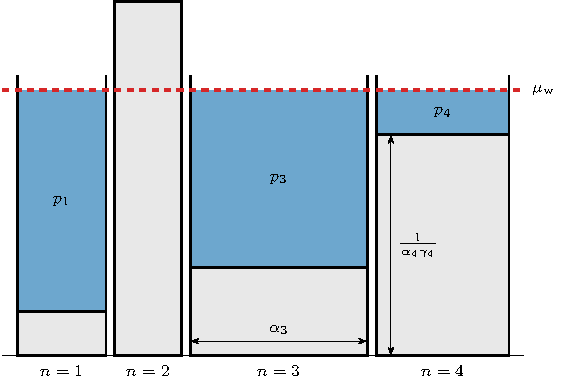
\includegraphics[width=0.625\textwidth]{figures/annex/A_waterfilling/out/waterfilling_algorithm.pdf}
    \caption[Waterfilling algorithm interpretation]{A visualization of the waterfilling algorithm for optimal power allocation strategy in a system with $N = 4$ channels.}
    \label{fig:waterfilling_algorithm}
\end{figure}

The complete procedure for determining the water level and the corresponding power allocation is summarized in Algorithm~\ref{alg:waterfilling}.
\begin{algorithm}[!htbp]
\caption{Waterfilling Algorithm for power allocation across Gaussian \ac{SISO} subchannels}
\label{alg:waterfilling}
\begin{algorithmic}[1]
    
    \Require 
    \Statex \hspace{-\algorithmicindent} \textbullet \, The total transmit power: $P_t$;
    \Statex \hspace{-\algorithmicindent} \textbullet \, The weight factor of each channel: $\alpha_n$ for $n = 1, \dots, N$;
    \Statex \hspace{-\algorithmicindent} \textbullet \, The ratios between channel gain and noise power: $\gamma_n = g^2_n / N_0$ for $n = 1, \dots, N$.
    
    \Ensure  The optimal power allocation $p_n$ for $n = 1, \dots, N$.

    \medskip
    \Statex \hspace{-\algorithmicindent}\textbf{Initialization:} Determine the width and height of all channel containers.
    \Statex \hspace{-\algorithmicindent} Find the permutation $\mathcal{P}: n \rightarrow i$ between the original index $n$ and the sorted index $i$ that sorts
    \Statex \hspace{-\algorithmicindent} the weighted ratios between channel gain and noise power $\alpha_n \gamma_n$ in decreasing order ($\mathrm{O}(N\log N)$).
    \State $w_i \leftarrow \alpha_{\mathcal{P}(n)}, \quad h_i \leftarrow 1 / (\alpha_{\mathcal{P}(n)} \gamma_{\mathcal{P}(n)})$
    
    \medskip
    \Statex \hspace{-\algorithmicindent}\textbf{Iteration:} Determine the optimal number of active channels ($\mathrm{O}(\log N)$).
    \State $N^{\mathrm{LB}}, \, N^{\mathrm{UB}} \leftarrow 0, \, N$
    \While{$N^{\mathrm{UB}} - N^{\mathrm{LB}} > 1$}
        \Statex \hspace{\algorithmicindent/2} Update the number of active channels: 
        \State  $N^{\mathrm{iter}} \leftarrow \left\lfloor (N^{\mathrm{UB}} + N^{\mathrm{LB}}) / 2 \right\rfloor$
        \Statex \hspace{\algorithmicindent/2} Compute the minimum power required to activate $N^{\mathrm{iter}}$ channels:
        \State  $P_{\mathrm{min}} \leftarrow \textstyle\sum_{i=1}^{N^{\mathrm{iter}}} w_i \left( h_{N^{\mathrm{iter}}} - h_i \right)$
        \Statex \hspace{\algorithmicindent/2} Update the bound on the number of active channels:
        \State  \textbf{if} $P_{\mathrm{min}} < P_t$ \textbf{then} $N^{\mathrm{LB}} \leftarrow N^{\mathrm{iter}}$ \textbf{else} $N^{\mathrm{UB}} \leftarrow N^{\mathrm{iter}}$
    \EndWhile
    
    \medskip
    \Statex \hspace{-\algorithmicindent}\textbf{Termination:} Compute the power allocated to each channel.
    \Statex \hspace{-\algorithmicindent} Fill the $N^{\mathrm{LB}}$ active stream containers:
    \State $p_i \leftarrow w_i \left(h_{N^{\mathrm{LB}}} - h_i\right)$ \quad for $i = 1, \dots, N^{\mathrm{LB}}$
    \Statex \hspace{-\algorithmicindent} Distribute the remaining power among the active channels according to their weight:
    \State $p_i \leftarrow p_i + (w_i / \textstyle\sum_{i'=1}^{N^{\mathrm{LB}}} w_{i'}) \cdot (P_t - \textstyle\sum_{i'=1}^{N^{\mathrm{LB}}} p_{i'})$ \quad for $i = 1, \dots, N^{\mathrm{LB}}$
    \Statex \hspace{-\algorithmicindent} Set the power of the inactive channels to zero:
    \State $p_i \leftarrow 0$ \quad for $i = N^{\mathrm{LB}} + 1, \dots, N$
    \Statex \hspace{-\algorithmicindent} Use the inverse permutation $\mathcal{P}^{-1}$ to map the allocated power back to the original index $n$.
    \State $p_n \leftarrow p_{\mathcal{P}^{-1}(i)}$
    
    \medskip
    \Statex \hspace{-\algorithmicindent}\textbf{Return} $p_n$ for $n = 1, \dots, N$

\end{algorithmic}
\end{algorithm}


\section{Examples}
\label{appendix_section:waterfilling_examples}
% =============================
%          Examples
% =============================

% Example 1: piecewise frequence selective channel
\paragraph{Piecewise Frequency-Selective Channel}~\\
Consider a channel with a piecewise constant frequency response, partitioned into $N$ non-overlapping subbands.
Subband $n$ spans the frequency interval $[B_{n-1}, B_n]$ and has a bandwidth $\beta_n = |B_n - B_{n-1}|$, a constant channel gain $g_n$, and experiences additive white Gaussian noise with power spectral density $N_0$.

The capacity of this channel can then be written as
\begin{subequations}
\label{eq:capacity_piecewise_frequency_selective_channel}
\begin{align}
    C
    &= \max_{|S(f)|^2} \int_f \log_2 \left( 1 + \frac{|H(f)|^2}{N_0} |S(f)|^2 \right) df
    \qquad \text{s.t.} \quad \int_f |S(f)|^2 df \leq P_t
    \label{eq:capacity_piecewise_frequency_selective_channel_1} \\
    &= \max_{|S(f)|^2} \sum_{n=1}^{N} \int_{B_{n-1}}^{B_n}
    \log_2 \left( 1 + \frac{g_n}{N_0} |S(f)|^2 \right) df
    \qquad \text{s.t.} \quad \int_f |S(f)|^2 df \leq P_t
    \label{eq:capacity_piecewise_frequency_selective_channel_2} \\
    &= \max_{p_n} \sum_{n=1}^{N} \beta_n \log_2 \left( 1 + \frac{g_n}{N_0} \frac{p_n}{\beta_n} \right)
    \qquad \text{s.t.} \quad \sum_{n=1}^{N} p_n \leq P_t
    \label{eq:capacity_piecewise_frequency_selective_channel_3}
\end{align}
\end{subequations}
where $S(f)$ denotes the power spectral density of the transmitted signal and $H(f)$ the frequency response of the channel.
In the final step, Jensen's inequality and the concavity of the logarithm imply that the capacity-achieving power spectral density is constant within each subband. Accordingly, if $p_n$ denotes the total power allocated to subband $n$, then $|S(f)|^2 = p_n / \beta_n$, for $f \in [B_{n-1}, B_n]$.

The optimization problem in~\eqref{eq:capacity_piecewise_frequency_selective_channel_3} is a special case of~\eqref{eq:optimal_power_allocation_optimization_problem} with $\alpha_n = \beta_n$ and $\gamma_n = g_n / (N_0 \beta_n)$.
Hence, the capacity-achieving power allocation can be obtained by applying the waterfilling algorithm described in the previous section.


% Example 2: SU-MIMO
\paragraph{Single-User MIMO Channel}~\\
As shown in Section~\ref{subsection:su_mimo_capacity}, a \ac{SU}-\ac{MIMO} channel can be decomposed into $R_H$ independent parallel \ac{SISO} eigen subchannels by means of the \ac{SVD} of the channel matrix.

The capacity optimization problem takes the form
\begin{equation*}
    C = \, \max_{\{p_n\}} \sum_{n=1}^{N_s} \log_2 \!\left( 1 + \frac{\sigma_n}{N_0} \, p_n \right)
    \qquad \text{s.t.} \quad \sum_{n=1}^{N_s} p_n \leq P_t,
\end{equation*}
where $p_n$ is the power allocated to the $n$-th eigen subchannel with channel gain $\sigma_n$ and $N_0$ is the noise power on each receive antenna.

This is a special case of~\eqref{eq:optimal_power_allocation_optimization_problem} with $\alpha_n = 1$ and $\gamma_n = \sigma_n / N_0$.
Hence, the optimal power allocation, in the sense that it achieves the capacity, can be obtained by applying the waterfilling algorithm described in the previous section.
